
\chapter{Introduction }
\paragraph{} Over the past decade, benefiting from the rapid
development of wireless communication technology, sensing
technology and the improvement of big data analysis
capacity [1], the Internet of Things (IoT) is growing with
incredible speed in most areas, especially in healthcare [2],
smart city [3] and autonomous vehicles [4]. As the essential
elements of the IoT world, data collected from various
devices can be applied in a wide range of areas after being
analyzed and processed. Combining with advanced
technologies such as big data and artificial intelligence [5],
IoT service based on data not only reduces the cost of
industry and agriculture and makes the devices around
people more intelligent, but also repeatedly optimizes the
IoT ecosystem (security, equipment management and the
standardization [6]) itself. However, due to the limited high
maintenance and management cost [7], restricted collecting
scope in privacy data, data exchange between individual and
organizations become irreversible trend when they realize
that connection is more important than possession [8].
Therefore, a lot of data exchange or sharing platform hava
emerged in the past years. Such as crawdad for archiving
wireless data [9], data science central provided industry’s
online resources for big data practitioners, data.gov as the
home of the US government’s open data platform, the
development of digital coast met the unique needs of the
coastal management community [10,11]. Most of them
concentrated on data of the same kind or a specific field and
led by government or the unions of large institutions.
However, the data sets on such centralized platform cannot
meet the public’s diversified demands, largely due to they
cannot provide enough trust to guarantee the transparency,
auditable, immutable in data exchange process.
\paragraph{}It has been watched by researchers for a long time, as the issue of trust kills the enthusiasm to share data actively and seriously hampers the development of the data industry [12]. Although current platforms integrate a lot of confidentiality
mechanisms (access control, authorization privacy) and
propose some trust model for data sharing in IoT, they are
not break away from the third party [13].
\paragraph{}In order to guarantee IoT data exchange in a completely
trusted, transparent environment, we propose a decentralized
solution based-on blockchain. As the core technology inBitcoin, blockchain soon came to be widely attracted
attention and application for its trust property[14].
\paragraph{}The core advantage of blockchain is decentralization. It consists of data encryption, timestamp, distributed consensus
algorithm, economic incentive mechanism and other
technology. It is applicable to the point-to-point transaction
based on decentralized credit in distributed systems without
mutual trust. Sequentially, this technology solves the
prevailing high cost, low efficiency and uneasiness of data
storage in current central institutions. This paper utilizes the feature of data is not tampered and completely transparent, combines with the time stamp and the transaction details in the process of storage and trading, so that it can be trusted by many parties. Its mixed encryption technology based on asymmetric encryption makes the user's privacy information
secure with the public and private key as the only identifier
of transaction subject. The second generation blockchain
introduces intelligent contract, which makes the blockchain
easier to use distributed application programming and speed
up transaction speed. The Ethereum intelligent contract
combined with capability-based access control method
makes the data provider can completely control their own
data sharing permissions quickly and efficiently and
completely solve the credible issues of original system in the
data.
\chapter{Little about the core technologies}
\section{Internet of Things(IOT)}
\subsection{what do IoT really Means?} 

\paragraph{}Definition - What does Internet of Things (IoT) mean?
The internet of things (IoT) is a computing concept that describes the idea of everyday physical objects being connected to the internet and being able to identify themselves to other devices. The term is closely identified with RFID as the method of communication, although it also may include other sensor technologies, wireless technologies or QR codes.
\paragraph{}The IoT is significant because an object that can represent itself digitally becomes something greater than the object by itself. No longer does the object relate just to its user, but it is now connected to surrounding objects and database data. When many objects act in unison, they are known as having ``ambient intelligence."
\paragraph{}The internet of things is a difficult concept to define precisely. In fact, there are many different groups that have defined the term, although its initial use has been attributed to Kevin Ashton, an expert on digital innovation. Each definition shares the idea that the first version of the internet was about data created by people, while the next version is about data created by things. In 1999, Ashton said it best in this quote from an article in the RFID Journal:\\
``If we had computers that knew everything there was to know about things using data they gathered without any help from us  we would be able to track and count everything, and greatly reduce waste, loss and cost. We would know when things needed replacing, repairing or recalling, and whether they were fresh or past their best."
\paragraph{}Most people think about being connected in terms of computers, tablets and smartphones. IoT describes a world where just about anything can be connected and communicate in an intelligent fashion. In other words, with the internet of things, the physical world is becoming one big information system.
\subsection{How it works?} 
\paragraph{}An IoT ecosystem consists of web-enabled smart devices that use embedded processors, sensors and communication hardware to collect, send and act on data they acquire from their environments. IoT devices share the sensor data they collect by connecting to an IoT gateway or other edge device where data is either sent to the cloud to be analyzed or analyzed locally. Sometimes, these devices communicate with other related devices and act on the information they get from one another. The devices do most of the work without human intervention, although people can interact with the devices -- for instance, to set them up, give them instructions or access the data.
\paragraph{}The connectivity, networking and communication protocols used with these web-enabled devices largely depend on the specific IoT applications deployed.
\begin{figure}[h]
	\centering
	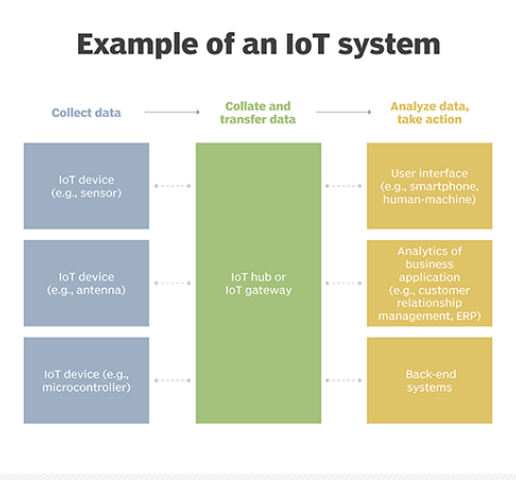
\includegraphics[width=8cm]{./iot_archi}
	\caption{IoT System}
\end{figure}

\subsection{Consumer and enterprise IoT applications}
\paragraph{}There are numerous real-world applications of the internet of things, ranging from consumer IoT and enterprise IoT to manufacturing and industrial IoT (IIoT). IoT applications span numerous verticals, including automotive, telco, energy and more.
\paragraph{}In the consumer segment, for example, smart homes that are equipped with smart thermostats, smart appliances and connected heating, lighting and electronic devices can be controlled remotely via computers, smartphones or other mobile devices.
\paragraph{}Wearable devices with sensors and software can collect and analyze user data, sending messages to other technologies about the users with the aim of making users' lives easier and more comfortable. Wearable devices are also used for public safety -- for example, improving first responders' response times during emergencies by providing optimized routes to a location or by tracking construction workers' or firefighters' vital signs at life-threatening sites.
\paragraph{}In healthcare, IoT offers many benefits, including the ability to monitor patients more closely to use the data that's generated and analyze it. Hospitals often use IoT systems to complete tasks such as inventory management, for both pharmaceuticals and medical instruments.
\begin{figure}[h]
	\centering
	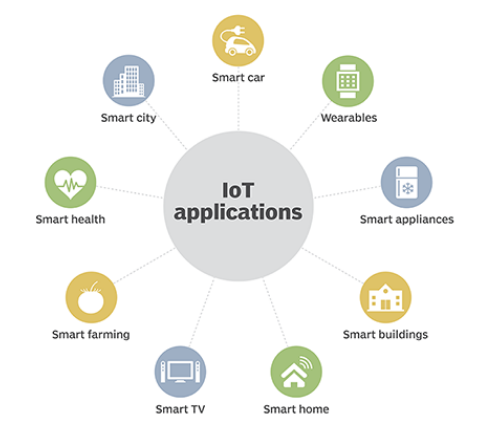
\includegraphics[width=9cm]{./iot_application}
	\caption{IoT Applications}
\end{figure}
\paragraph{}Smart buildings can, for instance, reduce energy costs using sensors that detect how many occupants are in a room. The temperature can adjust automatically -- for example, turning the air conditioner on if sensors detect a conference room is full or turning the heat down if everyone in the office has gone home.
\paragraph{}In agriculture, IoT-based smart farming systems can help monitor, for instance, light, temperature, humidity and soil moisture of crop fields using connected sensors. IoT is also instrumental in automating irrigation systems.
\paragraph{}In a smart city, IoT sensors and deployments, such as smart streetlights and smart meters, can help alleviate traffic, conserve energy, monitor and address environmental concerns, and improve sanitation.
\paragraph{} Components of IoT:
\begin{enumerate}
\item \textbf{Sensors/Devices:}\\
First, sensors or devices collect data from their environment. This could be as simple as a temperature reading or as complex as a full video feed.
\paragraph{}I use ``sensors/devices,” because multiple sensors can be bundled together or sensors can be part of a device that does more than just sense things. For example, your phone is a device that has multiple sensors (camera, accelerometer, GPS, etc), but your phone is not just a sensor.
\paragraph{}However, whether it`s a standalone sensor or a full device, in this first step data is being collected from the environment by something.
\item \textbf{Connectivity:}\\
Next, that data is sent to the cloud , but it needs a way to get there!
\paragraph{}The sensors/devices can be connected to the cloud through a variety of methods including: cellular, satellite, WiFi, Bluetooth, low-power wide-area networks (LPWAN), or connecting directly to the internet via ethernet.
\paragraph{}Each option has tradeoffs between power consumption, range and bandwidth (here’s a simple explanation). Choosing which connectivity option is best comes down to the specific IoT application, but they all accomplish the same task: getting data to the cloud.
\item \textbf{Data Processing:}\\
Once the data gets to the cloud, software performs some kind of processing on it.
\paragraph{}This could be very simple, such as checking that the temperature reading is within an acceptable range. Or it could also be very complex, such as using computer vision on video to identify objects (such as intruders in your house).
\paragraph{}But what happens when the temperature is too high or if there is an intruder in your house? That’s where the user comes in.
\item \textbf{User Interface:}\\
Next, the information is made useful to the end-user in some way. This could be via an alert to the user (email, text, notification, etc). For example, a text alert when the temperature is too high in the company’s cold storage.
\paragraph{}Also, a user might have an interface that allows them to proactively check in on the system. For example, a user might want to check the video feeds in their house via a phone app or a web browser.
\paragraph{}However, it’s not always a one-way street. Depending on the IoT application, the user may also be able to perform an action and affect the system. For example, the user might remotely adjust the temperature in the cold storage via an app on their phone.
\paragraph{}And some actions are performed automatically. Rather than waiting for you to adjust the temperature, the system could do it automatically via predefined rules. And rather than just call you to alert you of an intruder, the IoT system could also automatically notify relevant authorities.
\end{enumerate}

\section{Security Issue and vulnerabilities of IoT}
One of the security weakness of IoT is that it increases
the number of devices behind network’s firewall. As
Based on the review in, ten years ago, there was a
major concern about protecting computers, five years
ago, the concern was about protecting smartphones.
Now we have to worry about protecting our car, our
home appliances, our wearables, and many other IoT
devices. Computers also have security problems but
with automatic and easier updates have helped alleviate
this problem. But in case of IoT devices, manufacturers
are pressured to get their devices in the market , there
by ending up on compromising the security. Even if
they may offer firmware upgrades for a time, they often
stop when they focus on constructing the next device,
leaving customers with slightly outdated hardware that
can become a security risk.
\paragraph{}IoT devices have security concerns, as these devices can easily get attacked by hackers, the data will be
hacked and these devices may get controlled or accessed
by the hackers. The point is that we have to think about
what a hacker could do with a device if he can break
through its security. A strong cryptographic algorithms
are required to secure IoT devices and to provide secure
channel. The following lists different kinds of attacks
which have been observed recently and discussed in.
\subsection{DDoS attacks}
In 2016, the Mirai botnet launched one of the
biggest DDoS attacks ever recorded. More than 1
terabyte per second flooded the network of Dyn, a
major DNS provider, and brought down sites such as
Reddit and Airnbnb. But what made this attack so
special was that it was the first to be carried out with
IoT devices. Nearly 150,000 compromised smart
cameras, routers and other devices all enslaved into a
single botnet, focused on a single target.
\paragraph{}Manufacturers usually use a handful of default
password and usernames to protect an IoT device. So
there will be a few hundreds/thousands of password
combinations to protect tens of millions of smart
devices. All it took were a few simple lines of code,
designed to test each of those default passwords. A
device could be hacked and enslaved within a few
seconds, so long as the user didn’t change the standard
login information.
\subsection{ Unsecure car apps }
As Internet connected cars are coming around, it has
been observed that hackers are trying to take control of
the onboard software , trying to access and open the car
locks. Unsecure car apps can allow malicious
hackers to control one’s car.
\subsection{ Insecure default login credentials}
In practice, manufacturers might hide the “Change
password/Username” options deep in the UI, out of
sight for most users. If each Internet of Things device
had a randomized username and password, Mirai might
not have happened in the first place.
\subsection{Poor software updates}
Many Internet of Things manufacturers don’t even
patch or update the software that came on their devices.
If a device has software vulnerability, there’s little one
can done to prevent an attacker from exploiting it
without help from the manufacturer.
\subsection{The communication isn’t encrypted}
Many IoT devices lack basic encryption to hide the data
sent between the device and the central server. This can
potentially expose the user’s personal information, if a
malicious hacker can snoop in on his personal
information.
\paragraph{}Another thing that Internet of Things devices do, is that
some of them ask for more permissions than they need
to.One time, numerous Amazon Echo users were
surprised to see their device ordering dollhouses after a
TV anchor said the phrase “Alexa ordered me a
dollhouse”.In that case, the device had permission to do
a purchase all by itself. Each extra permission in an IoT
device adds another vulnerability layer which can be
exploited. The fewer permissions, the more secure your
device is.
\subsection{ Insecure user interface}
A device’s user interface is usually the first thing a
malicious hacker will look into for any vulnerabilities.
For instance, he might try to manipulate the “I forgot
my password”, in order to reset it or at least find out
your username or email.
\paragraph{}A properly designed device should also lock out a user
from attempting to login too many times. This
stops dictionary and brute force attacks that target
passwords, and greatly secures your device credentials.
In other cases, the password might be sent from the
device to the central server in plain text, meaning it isn’t
encrypted. 
\subsection{Poor privacy protection}
Internet connected devices are data-hungry beasts, but
some of them have a greater appetite than others. The
less information they have on you, the better, since it
limits how much a cybercriminal can learn about you if
he hacks the device. As a rule, try to look into what type
of data a device will store about you. Be critical of those
that harvest data they don’t need, such as coffee
machines storing user’s location information.
\section{Blockchain}
\subsection{Structure of a block}
A blockchain, is a growing list of records, called blocks, which are linked using cryptography.
Each block contains a cryptographic hash of the previous block, a timestamp, and transaction
data (generally represented as a merkle tree root hash). A block is a container data structure,
which brings together transactions for inclusion in the public ledger, known as the blockchain.
The block is made up of a header; containing metadata, followed by a long list of transactions. A
block can be identified in two ways, either by referencing the block hash, or through referencing
the block height. The block header consists of three sets of block metadata. Metadata is data
that provides information about other data. Firstly, there is a reference to a previous block
hash, which connects this block to the previous block, lying in the blockchain. The second set of
metadata relates to the mining competition; namely the difficulty, timestamp and nonce. Lastly,
the third piece of metadata is the Merkle Tree root; a data structure used to summarize all the
transactions in the block in an efficient manner.
\paragraph{}Block headers can be regarded as an example of a dynamic membership multi-party signature
(DMSS). A DMSS is a digital signature formed by a set of signers which has no fixed size
(Back, Corallo, Dashjr,
Friedenbach, 2014).Bitcoins block headers are DMSS because their
proof of work has the property that anyone can contribute without undergoing an enrolment
process. Furthermore, contribution is weighted by proportional computational power rather than one threshold signature contribution per party (Back, Corallo, Dashjr, Friedenbach, 2014).
\paragraph{}This allows anonymous membership without risk of a Sybil attack. A Sybil attack is when one
party joins many times and has an uneven, disproportionate input into the signature. Since the
blocks are chained together, Bitcoins DMSS is cumulative. A chain of block headers is also a
DMSS on its first block, with computational strength equivalent to the sum of the computational
strengths of the composing DMSS . Therefore, the key innovation in Blockchain is a signature of
computational power, rather than the typical signature of knowledge.
\begin{figure}[h]
	\centering
	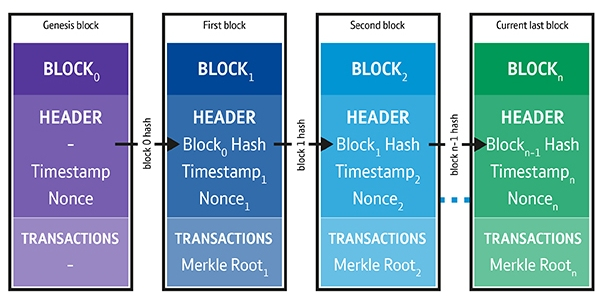
\includegraphics[width=9cm]{./blockchain-diagrams-02}
	\caption{Blockchain structure}
\end{figure}
\subsection{Block header hash and nodes}
Here I have am providing an example, the block hash of the first Bitcoin block ever created will
be like 000000000019d7789c085ae165831e934gf763ae46a4a6c172b3f1b60a8ce26f. The block hash
identifies a block uniquely, and can be independently derived by any node simply by hashing the
block header. A node is a full client. A full client is a client that owns the block chains and is
sharing blocks and transactions across the blockchain network. A node is considered to be part
of the blockchain infrastructure, and does not necessarily have to be a miner. Each node keeps
a complete copy of a totally ordered sequence of events in the form of a blockchain . The blocks
hash is computed by each node, as the block is received from the network. The block hash may
be stored in a separate database table as part of the blocks metadata, to facilitate indexing and
faster retrieval of blocks from disk.
\subsection{Block height}
Block height is another method to identify a block, this time through its position in the
blockchain. The first block ever created is at block height 0 (zero), and in the case of Bit-
coin, is the same block that was referenced by the block hash of the above block which is
000000000019d7789c085ae165831e934gf763ae46a4a6c172b3f1b60a8ce26f .Each subsequent block
added on top of that first block is one position higher in the blockchain, like boxes stacked one on
top of the other.Block height does not always identify a particular singular block. It is possible
for two or more blocks may have the same block height, both competing for the same position
in the blockchain.
\subsection{Genesis Block}
The first block in any blockchain is termed the genesis block. If you start at any block and
follow the chain backwards chronologically, you will arrive at the genesis block. The genesis
block is statically encoded within the client software, that it cannot be changed. Every node
can identify the genesis blocks hash and structure, the fixed time of creation, and the single
transactions within. Thus every node has a secure root from which is possible to build a trusted
blockchain on.
\subsection{Proof of Work}
In Proof of Work, in order for an actor to be elected as a leader and choose the next block to
be added to the blockchain they have to find a solution to a particular mathematical problem.
Given that the hash function used is cryptographically secure, the only way to find a solution to
that problem is by bruteforce (trying all possible combinations). In other words, probabilistically
speaking, the actor who will solve the aforementioned problem first the majority of the time is
the one who has access to the most computing power. These actors are also called miners.
It has been widely successful primarily due to its following properties:
\begin{enumerate}
\item It is hard to find a solution for that given problem
\item When given a solution to that problem it is easy to verify that it is correct.
\end{enumerate}
\paragraph{}Whenever a new block is mined, that miner gets rewarded with some currency (block reward,
transaction fees) and thus are incentivized to keep mining. In Proof of Work, other nodes verify
the validity of the block by checking that the hash of the data of the block is less than a preset
number.Due to the limited supply of computational power, miners are also incentivized not to
cheat. Attacking the network would cost a lot because of the high cost of hardware, energy, and
potential mining profits missed.
\subsection{Linking blocks in the blockchain}
Nodes maintain a copy of the blockchain locally, starting from the genesis block. The local copy of the blockchain constantly updates as new blocks are discovered and subsequently built on the chain. As a node receives information of incoming blocks from the network, it will validate these blocks first, then link them to the existing blockchain.
\paragraph{}The process to establish a link is as follows; a node will examine the incoming block header and look for the “previous block hash”. Looking at this incoming block, the node finds the “previous block hash” field, which contains the hash of its parent block. This hash is known to the node previously. Therefore, the node reasons that this new block is a child of the last block on the chain, and is the legitimate extension of the chain. The node adds this new block to the end of the chain, making the blockchain longer with a new height of the incoming block, now validated.
\subsection{Cryptographic Hash Algorithm}
The blockchain data structure is a back-linked list of blocks of transactions, which is ordered.
It can be stored as a flat file or in a simple database. Each block is identifiable by a hash,
generated using the SHA256 cryptographic hash algorithm on the header of the block. Each
block references a previous block, also known as the parent block, in the previous block hash
field, in the block header.A hash, also known in long form as cryptographic hash function, is a
mathematical algorithm that maps data of arbitrary size to a bit string of a fixed size. In the
case of SHA 256, the result is a string of 32 bytes. The resultant 32 bytes makes it effectively
impossible to reverse the output, since the function was designed to be a one-way function .
\paragraph{}The idea behind a hash functions use is to facilitate a thorough means for searching for data
in a dataset. The most basic form of hash function is any function that can be used to map
data of arbitrary size to data of fixed size. This output is a bit-string known as the hash value,
hash sum or hash code. The hash values can be stored in a tabular form known as a hash table
and is an efficient indexing mechanism; especially useful in search performance. Hash functions
are collision-free too. That means its impossible to find two messages that hash to the same
hash value. Therefore, when given a compact hash, one can confirm that it matches a particular
input datum. Blocks can be identified from their hash, serving two purposes; identification and
integrity verification.
\paragraph{}Bitcoin hashing function makes use of the SHA 256, applied twice. It generates an almost-
unique, fixed size 256-bit (32-byte) hash security. Large classes of hash functions are based on
a building block of a compression function .Each block contains the hash of its parent inside its
own header. There lays a chain going all the way back to the first block created, also known as
the genesis block, linked together by a sequence of hashes. The previous block hash field is inside
the block header and thereby the current block hash is dependent on the parent block hash.
The childs own identity changes if the parents identity changes. When the parent is modified in
any way, the parents hash changes. The parents changed hash necessitates an alteration in the
previous block hash pointer of the child. This in turn causes the childs hash to mutate, which
requires a change in the pointer of the grandchild, which in turn alters the grandchild and so on.
\paragraph{}This cascading effect ensures that, once a block has many generations succeeding it, it cannot
be changed without consequently forcing a recalculation of all the subsequent blocks. Because
such a recalculation would require an enormous amount of computation, the existence of a long
chain of blocks fortifies the Blockchains deep history to be immutable; a key feature of blockchain
technology security.
\begin{figure}[h]
	\centering
	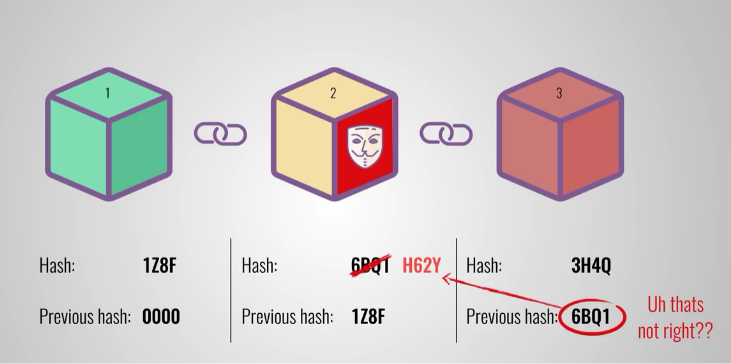
\includegraphics[width=9cm]{./block_change_hash}
	\caption{Denial on Data Modification}
\end{figure}
\subsection{Modification of Data}
By design, a blockchain is resistant to modification of the data. It is ”an open, distributed
ledger that can record transactions between two parties efficiently and in a verifiable and perma-
nent way”. For use as a distributed ledger, a blockchain is typically managed by a peer-to-peer
network collectively adhering to a protocol for inter-node communication and validating new
blocks. Once recorded, the data in any given block cannot be altered retroactively without al-
teration of all subsequent blocks, which requires consensus of the network majority. Although
blockchain records are not unalterable, blockchains may be considered secure by design and
exemplify a distributed computing system with high Byzantine fault tolerance. Decentralized
consensus has therefore been claimed with a blockchain.
\paragraph{}Blockchains are incredibly popular nowadays.Here, I have a chain of three blocks. As you can
see, each block has a hash and a hash of the previous block.So block 3 points to block 2 and
block 2 points to the block 1. Now the block 1 is special. It is the Genesis block and it cannot
point to any other block. Now if block 2 is tampered, it changes the hash of the block 2. Now
the hash in the block 3 becomes invalid as it does not match with the hash in the previous block.
Computers are very fast and they can calculate hash at a very high speed.
\chapter{Existing System Approach}
It relies on centralised, brokered communication models (also known as, client-server paradigm). All devices are identified, authenticated, and connected through cloud servers that sport huge processing and storage capacities. Connection among devices happen exclusively over the internet even if they’re a few feet apart. Also, machine-to-machine (M2M) communication is difficult because there is no single platform that connects all devices no guarantee that cloud services offered by different manufacturers are interoperable and compatible.

\paragraph{}The centralised architecture poses challenges to secure IoT deployments. Handling the enormous volume of existing and projected data is daunting. Managing the inevitable complexities of connecting to a seemingly unlimited list of devices is complicated. And the goal of turning the deluge of data into valuable actions seems impossible because of the many challenges. The existing security technologies will play a role in mitigating IoT risks but they are not enough. The goal is to get data securely to the right place, at the right time, in the right format; it’s easier said than done for many reasons.

\paragraph{}The centralised security model common in the enterprise today will struggle to scale up to meet the demands of the internet of things, or IoT.
\section{Disadvantages}
As most IoT networks are currently configured, data isn’t be considered trustworthy until it is vetted and allowed to pass through a single controlling security “gate.” As we saw with the Mirai incidents, a botnet barrage can focus efforts on compromising this lone point through a Distributed Denial of Service (DDNS) attack. Once through the centralized security “gate,” a hacker can access the resources of the entire IoT network. 
\begin{itemize}
	\item[]   \textbf{Online security:} Through something as ubiquitous as a coffee maker (or any of dozens of other devices) attached to a home network, a hacker could enter the system and gain access to ALL the information on ANY network connected device. That means passwords, checking or savings accounts – all the worst parts of identity theft. Following that thread of thought, it would be relatively easy to introduce ransomware or tell devices to stop functioning entirely.
	\item[] \textbf{Surveillance:} Got security cameras? Many homeowners and businesses do. One glaring weakness of a centralized server is how easy it is for hackers to get into the system and use security cameras to surveil the surroundings. What better way to have your privacy invaded or to case the place for a burglary? Even the remote camera on your vacuum cleaner could be hijacked by those with ill intent. We’re getting into creepy and legitimately dangerous territory here now.
	\item[] \textbf{ A large enterprise nightmare:} We’ve already mentioned Mirai. One offshoot, Persirai, has been trained to infect 1,250 different types of security cameras. As in the Mirai attack, the resources of a company’s network can be conscripted in support of a global DDNS attack. Since resources are involved in doing the hacker’s criminal bidding, there will be little bandwidth and processing left for legitimate work, slowing operations to a crawl and, oh, by the way, leaving protected company data wide open for stealing.
	\item[] \textbf{Shut it down:} Sometimes a hacker has no other end in mind than the mischief involved in making another person’s life miserable. There are so many ways to penetrate what passes for security in today’s IoT networks – Man in the Middle, spoofing, cloning, data sinkholes – that a bad actor can sit back and take his or her pick. Once inside, it’s an easy matter to shut down or destroy devices, infect them with malicious code, and make a network permanently unusable. When you might have spent thousands of dollars to create this “smart” home network in the first place, losing it all just because some tech whiz was bored on a Sunday afternoon is likely not your definition of a good time.
\end{itemize}
\chapter{Proposed System}
Blockchain technology can be used in tracking billions of connected devices, enable the processing of transactions and coordination between devices; allow for significant savings to IoT industry manufacturers. This decentralised approach would eliminate single points of failure, creating a more resilient ecosystem for devices to run on. The cryptographic algorithms used by blockchains, would make consumer data more private.

\paragraph{}The ledger is tamper-proof and cannot be manipulated by malicious actors because it doesn’t exist in any single location, and man-in-the-middle attacks cannot be staged because there is no single thread of communication that can be intercepted. Blockchain makes trustless, peer-to-peer messaging possible and has already proven its worth in the world of financial services through cryptocurrencies such as Bitcoin, providing guaranteed peer-to-peer payment services without the need for third-party brokers.

\paragraph{}The decentralized, autonomous, and trustless capabilities of the blockchain make it an ideal component to become a fundamental element of IoT solutions. It is not a surprise that enterprise IoT technologies have quickly become one of the early adopters of blockchain technologies.

\paragraph{}In an IoT network, the blockchain can keep an immutable record of the history of smart devices. This feature enables the autonomous functioning of smart devices without the need for centralized authority. As a result, the blockchain opens the door to a series of IoT scenarios that were remarkably difficult, or even impossible to implement without it.

\paragraph{}By leveraging the blockchain, IoT solutions can enable secure, trustless messaging between devices in an IoT network. In this model, the blockchain will treat message exchanges between devices similar to financial transactions in a bitcoin network. To enable message exchanges, devices will leverage smart contracts which then model the agreement between the two parties.

\paragraph{}One of the most exciting capabilities of the blockchain is the ability to maintain a duly decentralised, trusted ledger of all transactions occurring in a network. This capability is essential to enable the many compliance and regulatory requirements of industrial IoT applications without the need to rely on a centralised model.

\section{Combining blockchain and IoT}
There are several clear advantages to the idea of building smart machines able to communicate and operate via blockchain.

\paragraph{}Firstly, there is the issue of oversight. With data transactions taking place between multiple networks owned and administered by multiple organizations, a permanent, immutable record means custodianship can be tracked as data, or physical goods, pass between points in the supply chain. Blockchain records are by their very nature transparent — activity can be tracked and analyzed by anyone authorized to connect to the network.

\paragraph{}If something goes wrong, breakages occur, data leaks where it shouldn’t, then the blockchain record makes it simple to identify the weak link and, hopefully, take remedial action.

\paragraph{}Secondly, the use of encryption and distributed storage means that data can be trusted by all parties involved in the supply chain. Machines will record, securely, details of transactions that take place between themselves, with no human oversight.

\paragraph{}Without the private keys giving write-access to the blockchain (which in this case would be held by machines), no human will be able to overwrite the record with inaccurate information.

\paragraph{}Thirdly, the “smart contract” facilities provided by some blockchain networks, such as Ethereum, allow the creation of agreements which will be executed when conditions are met. This is likely to be highly useful when it comes to, for example, authorizing one system to make a payment, when conditions indicate that delivery of a service has been provided.

\paragraph{}Fourthly, blockchain offers the potential of greatly improving the overall security of the IoT environment. Much of the data generated by IoT is highly personal — for example, smart home devices have access to intimate details about our lives and daily routines. This is data that needs to be shared with other machines and services in order to be useful to us. But it also means there are far more openings for hackers to potentially attack us. Business and governments invested in IoT also have to contend with this increased scope for a data breach by criminals, rivals or foreign enemies.

\paragraph{}Above the fact that it will offer new opportunities, it is even possible that blockchain and IoT convergence will become a necessity at some point. If the current IoT paradigm — devices connected via a centralized cloud storage and processing service — continues, then systems are likely to become increasingly bloated, as data volumes, as well as the number of connected devices, continue to increase.

\paragraph{}These cloud services are likely to become bottlenecks as the amount of data pumped through them increases. Blockchains can remedy this thanks to their distributed nature. Rather than an expensive, centralized data center, a blockchain data storage network is duplicated across the hundreds (or potentially thousands, or millions) of computers and devices which make up the network. This huge amount of redundancy means data will always be close at hand when it’s needed, cutting down transfer times and meaning one server failure will be of no consequence to business activity.

\section{Advantages}
Four ways IoT can exploit blockchain technology:
\begin{enumerate}
\item Trust building
\item Cost reduction
\item Accelerated data exchanges
\item Scaled security
\end{enumerate}
Here are some ways the distributed architecture of blockchain can help solve many of these security and trust challenges:
\begin{itemize}
\item Blockchain can be used to track the sensor data measurements and prevent duplication with any other malicious data.

\item Deployments of IoT devices can be complex, and a distributed ledger is well suited to provide IoT device identification, authentication and seamless secure data transfer.

\item Instead of going through a third party for establishing trust, IoT sensors can exchange data through a blockchain.

\item A distributed ledger eliminates a single source of failure within the ecosystem, protecting a IOT device data from tampering.

\item Blockchain enables device autonomy (smart contract), individual identity, integrity of data and supports peer to peer communication by removing technical bottlenecks and inefficiencies.

\item The deployment and operation costs of IoT can be reduced through blockchain since there is no intermediary.

\item IoT devices are directly addressable with blockchain, providing a history of connected devices for troubleshooting purposes.
\end{itemize}

\chapter{ Trusted Requirements}
IoT data as a special commodity, is collected by
government, corporations, even individual, which are of
great value to different application fields. Such owner needs
a trusted platform to exchange their IoT data in order to
improve data utilization and benefit from the trade. We
divided data exchange needs for trust into three categories.
\section{Trusted Trading}
Trusted Trading requirement means the whole
transaction process is recorded and can not be modified by
either party if once confirmed. Besides, the detail transaction
history should be traceable by public.
In brief, the requirement of such trusted trading
requirement mainly includes accurate transaction description,
traceable and immutable transaction process. Some existing
solutions can record the trading history and provide
convenient searching function, even use distributed cloud
storage system to protecte the system from single point
failure problem . However, such systems were developed
and maintained by third-party organization which can not
guarantee the transaction record from maliciously modified.
Unlike the common system, blockchain based system
stored the exchange data in completely distributed peer to
peer network . It ensures the data on blockchain can not
be arbitrarily changed and can audit according to time order.
In addition, the blockchain node can be downloaded by
anyone, so the exchange data is transparent [18]. At the same
time, the chain of blockchain information is completely
transparent, so the data transaction information can be
completely symmetric compared with traditional trading
platform.
\section{Trusted Data Access}
Trusted Data Access requirement means data owner can
hold their ownership, even can be realized personalized
empower the access right after exchange IoT data [19].
Current platforms need the data providers upload their
data set to website or special cloud. So that the user cannot
hold the access permission of their data set after send to
third-party organization and don’t know who access their
data. In our solution, we separate the data exchange into two
parts: origin data exchange and data access right exchange.
Origin data exchange way is customized by data provider,
and can be verified by the data access right store on
blockchain which protected by consensus mechanism.
Adopting various safety related technologies of block chain
to jointly safeguard the security of data access and the rights
of the data owner during transaction. Meanwhile, the full
distribution characteristics of the blockchain can also make
the access verification of permissions more convenient.
\section{Trusted Privacy Preserve}
Trusted Privacy Preserve requirement mean data owner
can protect their personal information while data exchange.
Because some IoT data regarding privacy matters are not the
data requesters’ concerns.
In third-party data exchange platform, users should
provide some personal information even binding the credit
card at registration time. Such privacy is vulnerable to
hijacking by others and some IoT data also can reflect living
habits of individuals. So privacy also preserves a pressing
need in IoT data exchange .
Blockchain as an anonymous network, use 64-bit address
to identify users which generated by RSA and protected by
SHA-256. Participants send transactions only with public
address without any personal information, so that the privacy
preserve can be trusted .


\chapter{ Architecture}

The IoT data exchange framework based on blockchain
is a decentralized application platform in which user can
trade data in trusted environment. The framework can be
divided into Data Layer, Network Layer, Protocol Layer and
Interaction Layer. Figure shows the overall architecture.
\begin{figure}[h]
	\centering
	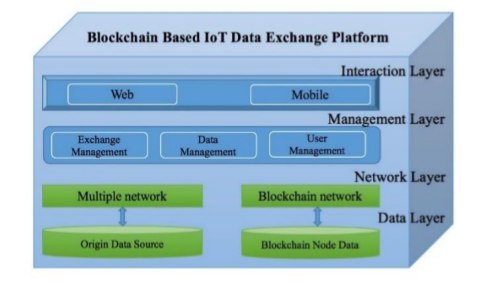
\includegraphics[width=9cm]{./architecture}
	\caption{Architecture of blockchain based IoT data exchange platform}
\end{figure}
\section{Data Layer}
Data layer consists of two parts: the IoT data and the
exchange data. The former can be stored in various places as
data source, such as storage clouds, database clouds, even
wireless sensor network nodes which was managed by the
owner. Exchange data stored in blockchain network which
use to record the whole data exchange process. Exchangeparties are able to choose the data access methods and
personal customization storage medium which make them
feel appropriate, such as peer-to-peer transmission, access
online database with limited permissions, and even hard disk.
Exchange data includes the description of provide data or
data requirement, conditions of data exchange and the data
access authority.
Figure 1. Architecture of blockchain based IoT data exchange platform
\section{Network Layer} 
Network layer includes multiple network and blockchain
network [22]. Multiple network is responsible for origin data
access and transmission which form customized by the needs
of the individual. Typical access methods include
peer-to-peer network, personal website, and storage cloud.
Blockchain network composed of one or more blockchain
nodes that storage completely identical transactions
happened in such network [23]. As the core of the
architecture, the encryption and decentralized consensus
mechanisms of blockchain guarantee IoT data exchange in a
reliable, transparent and tamper-resistant environment.
\section{Management Layer}
Management layer is mainly responsible for common
management function of IoT data exchange. User
management controls the user’s security and permissions for
the platform. Data management is in charge of data
collecting and quick search by data attribute. Exchange
management as the core function of data exchange process,
will manage the data access right, exchange relationship
even records the transaction history.
\section{Interaction Layer}
Interaction layer provides the interface for data exchange
parties to communicate with each other. According to the
current mode of interaction, we separate them into two
pieces: web based interactions and mobile based interactions.
Web-based usually provides visual interfaces on website
while mobile based provides more common to packaging
into a app running on mobile phone, tablet even other
embedded device.
\chapter{ Major component design}
To increasing the degree of automation and system
configurable, we design a set of smart contracts for the major
management functions. Figure shows the architecture of smart
contract based management component
\begin{figure}[h]
	\centering
	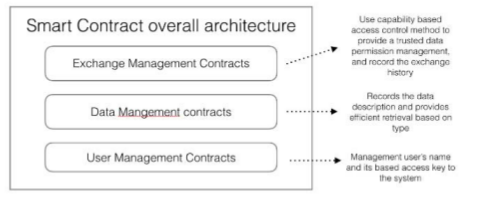
\includegraphics[width=9cm]{./smatcontract_management}
	\caption{Architecture of smart contract based management component}
\end{figure}
\section{Exchange Management Contracts}
Exchange management contracts include three types
protocols: access contracts, communication contracts and
auto exchange contracts. Access contracts use capability
based access control method to provide a trusted data
permission management. Communication contracts record
the whole communicated process in IoT data exchange for
traceability. Auto exchange contracts will automatically send
the data access right to demander while they satisfy the
condition.
\paragraph{}Access contracts implement capability-based data access control method, including two functions of the data access
identifier generation and the data access rights exchange.
The data identification contract assigns a Data Access Ticket
to the data after the data owner has registered the data,
Referred to as "DAT”. Through this identifier, the user can
obtain access way and access permissions of the data. The
data access rights exchange contract is responsible for setting
data provision conditions and implementing automated
transaction. We assume that the data provider sets the
conditions set as Condition1, Condition2, for short C1, C2.
The contract will automatically provide DAT to the
demander when the data demanders send data to the contract
for a request for a transaction and the transaction satisfies C1, C2ˈand put the demanders in the list of authorized access to
that data. When users get access, they can download the
source data by means of URL or FTP or P2P seeds.
Communication contracts are determined by data, data
demanders, and data providers, and record all transaction
records between the three. When a data demander sends a
request or a negotiation to the contract, two parameters of the
data name and data provider are required. And vice versa, the
contract will be notified to both parties.
\section{Data Management Contracts}
Data management contracts include data contracts and
classified search contracts. When the data provider registers
data, the data contract will generate a separate corresponding
data object contract, which records the basic description of
the data (Such as name, attribute, data provider), and call the
data access contract method to generate data access identifier
at the same time. In order to improve the search efficiency,
we use the basic principle of hash table to perform secondary
classification for data, and design an extensible andcustomizable classifications. Data classification contracts
include data type management and data type corresponding
to the data set about management. Data type management is
responsible for generating and modifying Type Contract, and
the Data Type Contract is responsible for recording all data
object Contract address as pointer of this type. The user
invokes the contract and passes in the type parameter, which
can quickly get the data set of the corresponding type.
\section{User Management Contracts}
User management contracts as the basic contracts control
the user’s security and permissions of the platform by
maintaining the user-nickname relationship and user-role
relationship. User can use their nickname to communicate
with others facilitate the identification rather than 64-bit
address. The platform contains three main user roles: user
provider, user demander and auditor. Role contracts maintain
the user-role list used to defined responsibilities. The user's
interaction in the system uses the user alias and password, so
it can avoid privacy leak and better protect users' privacy.
